\lecture{2024-08-26}{Fractional cascading and range trees}

\textbf{Midterm 1:} September 9th. \\
\textbf{Homework 1} will be posted by Wednesday.

\begin{question*}
    Let $L_1, L_2, \dots, L_t$ be $t$ sorted lists, with
    $\sum_{i=1}^t \abs{L_i} = n$.
    Given a query $q$, report the successor of $q$ in each list.
\end{question*}
The naive binary search approach is $O(t \log n)$, but with
some preprocessing we can better this to $O(\log n + t)$.

\begin{definition}
    For any list $L$, we define $\onm{Even}(L)$
    to be the list of all even-indexed elements of $L$.
\end{definition}

\begin{solution}
    For each $i$ we define the list $L_i'$ as follows.
    \begin{align*}
        L_t' &= L_t \\
        L_i' &= \onm{merged}(L_i, \onm{Even}(L_{i+1}'))
    \end{align*}
    For example, if \begin{align*}
        L_1 &= \begin{bmatrix}
            2 & 3 & 7 & 16 & 19 & 32 & 36 & 37 & 48 & 51
        \end{bmatrix} \\
        L_2 &= \begin{bmatrix}
            15 & 25 & 30 & 35 & 40 & 45
        \end{bmatrix} \\
        L_3 &= \begin{bmatrix}
            5 & 10 & 17 & 20 & 27 & 50
        \end{bmatrix}
    \end{align*} then \begin{align*}
        L_3' &= \begin{bmatrix}
            5 & 10 & 17 & 20 & 27 & 50
        \end{bmatrix} \\
        L_2' &= \begin{bmatrix}
            10 & 15 & 20 & 25 & 27 & 30 & 35 & 40 & 45
        \end{bmatrix} \\
        L_1' &= \begin{bmatrix}
            2 & 3 & 7 & 15 & 16 & 19 & 25 & 30 & 32 \\ 36 & 37 & 40 & 48 & 51
        \end{bmatrix}
    \end{align*}
    Let us formally show that the sum of the new lengths is still $O(n)$.
    \begin{align*}
        \abs{L_t'} &= \abs{L_t} \\
        \abs{L_{t-1}'} &\le \abs{L_{t-1}} + \frac12 \abs{L_t} \\
        \abs{L_{t-2}'} &\le \abs{L_{t-2}} + \frac12 \abs{L_{t-1}'} \\
        &= \abs{L_{t-2}} + \frac12 \abs{L_{t-1}} + \frac14 \abs{L_t} \\
        \abs{L_{t-i}'} &\le \abs{L_{t-i}} + \frac12 \abs{L_{t-i+1}'} \\
        &= \abs{L_{t-i}} + \frac12 \abs{L_{t-i+1}} +
            \frac14 \abs{L_{t-i+2}} + \dots + \frac{1}{2^i} \abs{L_t}
    \end{align*}
    Thus the sum of lengths is \[
        \sum_i \abs{L_i'} < 2 \sum_i \abs{L_i}
    \]
    Call the elements that have cascaded up ($\onm{Even}(L_{i+1}')$) the
    \emph{cascaders}.

    While merging $L_i$ with $\onm{Even}(L_{i+1}')$, store a pointer,
    which we will call the \emph{cascader pointer},
    from each element $x \in L_i'$ to the largest element $\le x$ in
    $\onm{Even}(L_{i+1}')$.
    In our example, we store the pointers
    \begin{center}
        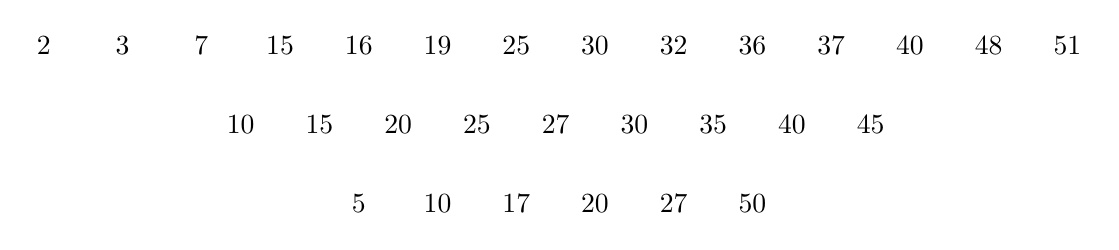
\begin{tikzpicture}
            \foreach \i/\x in {1/2, 2/3, 3/7, 4/15, 5/16, 6/19, 7/25, 8/30, 9/32, 10/36, 11/37, 12/40, 13/48, 14/51} {
                \node at (\i, 0) {$\x$};
            }
            \foreach \i/\x in {1/10, 2/15, 3/20, 4/25, 5/27, 6/30, 7/35, 8/40, 9/45} {
                \node at (\i+2.5, -1) {$\x$};
            }
            \foreach \i/\x in {1/5, 2/10, 3/17, 4/20, 5/27, 6/50} {
                \node at (\i+4, -2) {$\x$};
            }
            % \draw[->,thin] (4, 0) edge (2, -1);
                % (5, 0) -- (2, -1)
                % (6, 0) -- (2, -1)
                % (7, 0) -- (4, -1)
                % (8, 0) -- (4, -1)
                % (9, 0) -- (6, -1)
                % (10, 0) -- (6, -1)
                % (11, 0) -- (6, -1)
                % (12, 0) -- (7, -1)
                % (13, 0) -- (8, -1)
                % (14, 0) -- (9, -1)
                % (14, 0) -- (9, -1)
                % (3, -1) -- (1, -2)
                % (4, -1) -- (2, -2)
                % (5, -1) -- (2, -2)
                % (6, -1) -- (3, -2)
                % (7, -1) -- (3, -2)
                % (8, -1) -- (4, -2)
                % (9, -1) -- (5, -2);
        \end{tikzpicture}
    \end{center}
\end{solution}

\section{Back to range trees} \label{sec:back-to-2-d-range-trees}
$2$-D range trees store a sorted list or balanced binary search tree
at each node.
We can adapt fractional cascading to $2$-D range trees.
Since all internal lists are to be queried by the same $y$-coordinates
$y_1$ and $y_2$, this allows us to shave off one log factor.

For $d$-dimensional range trees, which ultimately contain $2$-D range trees
at some level, this still reduces one log factor.
Thus the total time complexity is $O(\log^{d-1} n + k)$.
